\chapter{Hiding and Attacking Strategies}
\label{cha:STRATEGIES}

As we all know , there are two tasks everyone robot / program should be able to complete on the vision simulator. First, Your robot chases the opponent robot and tries to hit it with the laser while the other robot tries to avoid getting hit. Second, The opponent robot chases your robot and tries to hit it with the laser while your robot tries to avoid getting hit. We find that obstacles are considered to block the laser so we give the following hiding and attacking strategies. 


\section{Hiding}
\begin{figure}[thb]
    \centering
    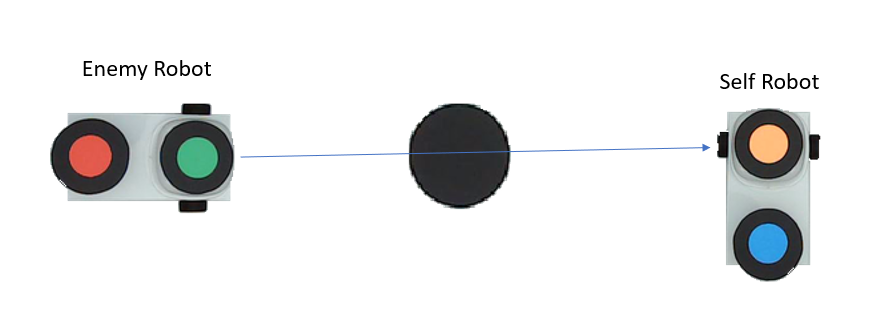
\includegraphics[width=0.4\textwidth]{images/hiding_strategy.png}
    \caption[hiding strategy]{an example of positions that satisfies the hiding strategy.}\label{hiding_strategy}
\end{figure}

In order to find the nearest point that satisfies the condition, an obstacle between the self and enemy, the foot of perpendicular from current position to the straight-line connecting enemy and obstacles, as shown in figure \ref{hiding_implement1}

\begin{figure}[thb]
    \centering
    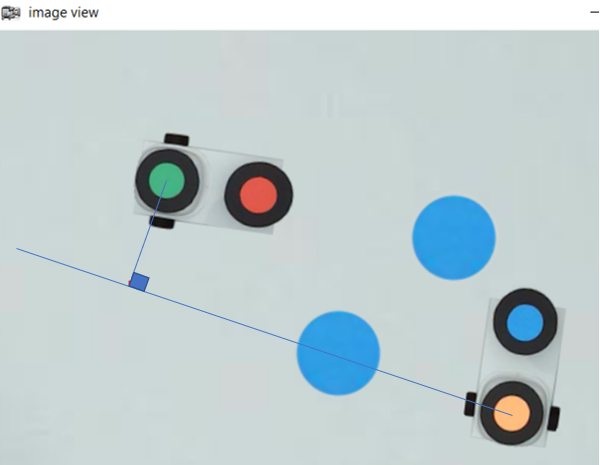
\includegraphics[width=0.4\textwidth]{images/implementofhiding1.png}
    \caption[he foot of perpendicular from current position to the straight-line connecting enemy and obstacles]{the foot of perpendicular from current position to the straight-line connecting enemy and obstacles.}\label{hiding_implement1}
\end{figure}

The calculation of the foot of the perpendicular is as follows:
We assume that $A=(x_{a},y_{a})$ ,  $B=(x_{b},y_{b})$ are position of enemy and obstacle as shown in figure \ref{hiding_implement2}. $C=(x_{c},y_{c})$ is the position of self-robot, $O=(x_{o},y_{o})$ is the foot of perpendicular from point $C$ to line $AB$.

\begin{figure}[thb]
    \centering
    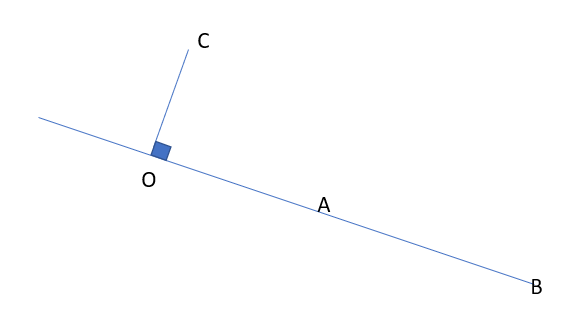
\includegraphics[width=0.4\textwidth]{images/implementofhiding2.png}
    \caption[The foot of perpendicular]{The foot of perpendicular.}\label{hiding_implement2}
\end{figure}
Since $\overrightarrow{AB} \perp  \overrightarrow{CO}$, we have:

\begin{equation}
(x_{b}-x_{a})(x_{o}-x_{c})+(y_{b}-y_{a})(y_{o}-y_{c})=0
\end{equation}

Since $\overrightarrow{AB}$ and $\overrightarrow{AO}$ has same direction, we have:
\begin{equation}
\left\{\begin{matrix}
x_{o}=k({x_{b}}-{x_{a}})+{x_{a}}\\
y_{o}=k({y_{b}}-{y_{a}})+{y_{a}}
\end{matrix}\right.
\end{equation}

Substitute $x_o$ and $y_o$ in the second equation to find out $k$. Then substitute $k$ in the third equation to find out $x_o$ and $y_o$.
\begin{equation}
    k=-\frac{(x_{a}-x_{c})(x_{b}-x_{a})+(y_{a}-y_{c})(y_{b}-y_{a})}{(x_{b}-x_{a})^{2}+(x_{b}-x_{a})^{2}}
\end{equation}

Once we have arrived at the expected position, direction of the self-robot is also important. As shown in figure \ref{hiding_implement3} a, if the direction of self-robot is not opposed to the enemy-robot, to run away from the enemy, the self-robot should rotate first, and then move around the obstacle. However, if we keep the direction of self-robot as opposed to the enemy, as shown in figure \ref{hiding_implement3} b, we do not need to rotate robot first, we can move robot around the obstacle directly instead.
\begin{figure}[htbp]
\centering
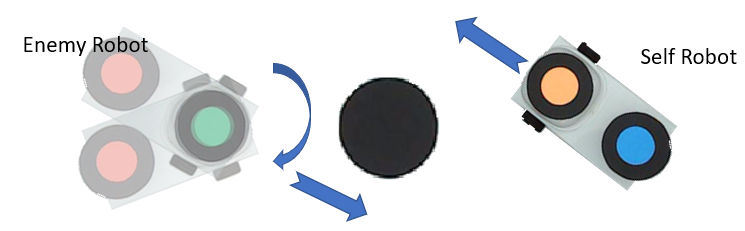
\includegraphics[width =0.4\textwidth]{images/implementofhiding3-1.png}
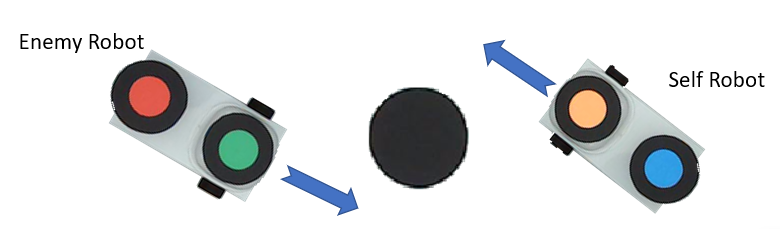
\includegraphics[width =0.4\textwidth]{images/implementofhiding3-2.png}
\caption{The importance of self-robot direction}\label{hiding_implement3}
\end{figure}

Therefore, to keep the direction as opposed to the enemy, the expected position also requests a specific theta.  For the convenience of calculation, we should stipulate that the theta of robot is between pi and -pi.





\section{Attacking}
Since there is only one chance to fire the laser, it should fire until there is no obstacle between two robots. To do so, the attacking robot should chase the other robot. We defined the criteria to fire the laser when:
\begin{itemize}

  \item The laser is pointing to one of the enemy robot’s centroids
  \item There is a free path (no obstacles) between the laser position and the enemy robot.
\end{itemize}
Inside the while loop, a series of conditions are programmed to check if the robot can fire the laser. For the first condition, the laser will be tracking the nearest enemy’s centroid. Figure \ref{laser_track} shows the distances measured by the program. These distances are compared and the smallest one is provided to the laser track algorithm. This function is just a simple adjustment to the laser's servo motor according to the error angle between the laser and the centroid location measured in the image frame. The function will output the error angle for the first condition to be met.

\begin{figure}[thb]
    \centering
    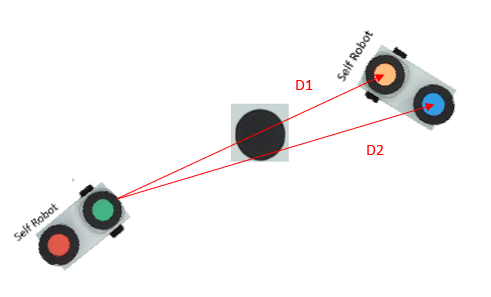
\includegraphics[width=0.5\textwidth]{images/laser_track.png}
    \caption[laser tracking]{Laser tracks the smallest distance to the robot's enemy}\label{laser_track}
\end{figure}

The second condition is met when there is no obstacles in the laser's path. Once the nearest centroid is chosen, the freepath() function will check if the laser is passing through an obstacle or not. This function keeps track of the pixels that are in between the laser and the enemy's chosen centroid. Then, the function checkspace() will tell if the pixel is an obstacle or not.\\
When condition one and condition two are met, the robot will laser the fire to the oponent.

To meet these conditions, the robot has to find a proper location with respect to the enemy. The strategy consists on chasing the enemy's closest centroid. This is done by using the mentioned path planning algorithm which finds the best trajectory while avoiding obstacles. When the described conditions are met, the robot will be able to fire the laser to the enemy.

